\documentclass[10pt]{beamer}

%-------------------------------------------------
%   THEMES & PACKAGES
%-------------------------------------------------
\usetheme[progressbar=frametitle]{metropolis}
\usepackage{graphicx}
\usepackage{booktabs}       % Nicer tables
\usepackage{hyperref}
\usepackage{subcaption}

%-------------------------------------------------
%   TITLE
%-------------------------------------------------
\title{Learning and Adaptivity}
\subtitle{Project presentation}
\date{Due date: June 21, 2016}
\author{Minh Nguyen}
\titlegraphic{\hfill
\includegraphics[height=0.7cm]{../../images/h-brs-logo.jpg}}

%-------------------------------------------------
%   BEGIN
%-------------------------------------------------
\begin{document}

%-------------------------------------------------
\maketitle

%-------------------------------------------------
%   WHAT
%-------------------------------------------------
\begin{frame}{Data set}
    \begin{alertblock}{Rossmann stores sales data}
        \href{https://www.kaggle.com/c/rossmann-store-sales/data}{Rossmann dataset} from Kaggle contains historical sales data for 1,115 Rossmann stores.
        \begin{figure}[t!]
            \begin{subfigure}[t]{0.5\textwidth}
                \centering
                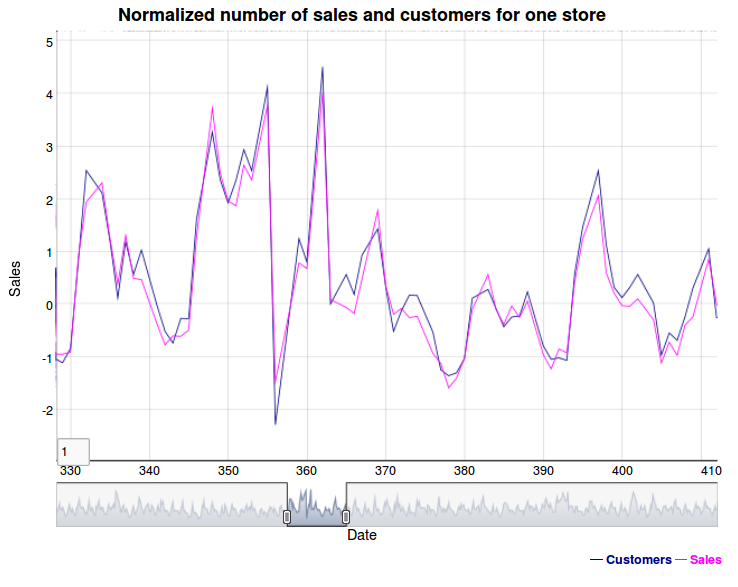
\includegraphics[height=1.5in]{rossmann_visualization_sales-customers}
                \caption{Normalized sales and customer number for one store}
            \end{subfigure}%
            \begin{subfigure}[t]{0.5\textwidth}
                \centering
                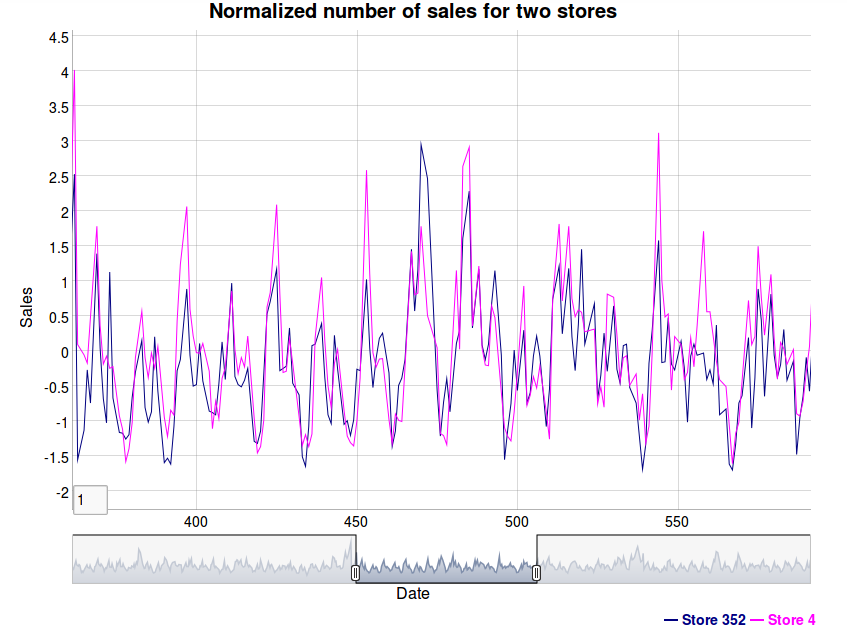
\includegraphics[height=1.5in]{rossmann_visualization_two-stores}
                \caption{Normalized sales for two stores}
            \end{subfigure}
            \label{fig:sub1}
            \end{figure}
        \end{alertblock}
\end{frame}

\begin{frame}{Data set}
    \begin{table}
        \centering
        \resizebox{\textwidth}{!}{%
            \begin{tabular}{llllllllll}
                \toprule
                \textbf{Feature} & Store & Sales & Customers & Date & DayOfWeek & Open & Promo & StateHoliday & SchoolHoliday\\
                \midrule
                \textbf{Type} &  integer & float & integer & date & integer & boolean  & boolean  & boolean & boolean\\
                \bottomrule
            \end{tabular}
        }
        \caption{Features from the train set}
        \end{table}

    \begin{table}
        \centering
        \resizebox{\textwidth}{!}{%
            \begin{tabular}{llllllll}
                \toprule
                \textbf{Feature}  & StoreType   & Assortment & Comp. Distance & Comp. OpenSince & Promo2  & Promo2Since & PromoInterval\\
                \midrule
                \textbf{Type}     & categorical & float      & float          & integer         & boolean & integer     & list of int \\
                \bottomrule
            \end{tabular}
        }
        \caption{Features from the store set}
    \end{table}

\end{frame}

%-------------------------------------------------
%   WHY
%-------------------------------------------------
\begin{frame}{Preprocessing}
    \begin{alertblock}{Missing values}
        \begin{itemize}
            \item Many stores do not have information on competitor, or does not participate in Promo2.
            \item Missing values for competitor's time of opening and time since Promo2 began are filled with zeros.
        \end{itemize}
    \end{alertblock}

    \begin{alertblock}{Additional features}
        \begin{itemize}
            \item ``open-since'' features are converted to the smallest time unit (i.e. 1 year 3 months is 15 months)
            \item ``WeekOfYear'' is added to capture seasonal trends in shopping
            \item Store IDs also used to better recognize different stores while combining data from multiple stores in training
        \end{itemize}
    \end{alertblock}

    \begin{alertblock}{Normalization}
    \end{alertblock}
\end{frame}

%-------------------------------------------------
%   WHY
%-------------------------------------------------
\begin{frame}{Method}
    \begin{alertblock}{RNN}
        \begin{itemize}
            \item samples from the network’s output distribution, then feeding the sample as input for the next time step
            \item suffers from vanishing or exploding gradients, can't store information for a long time
        \end{itemize}
    \end{alertblock}
    \begin{alertblock}{LSTM}
        Uses a gated mechanism in each hidden unit of RNN to better store memory
        \begin{itemize}
            \item input gates: when to update memory cell from inputs
            \item output gates: when to release information from memory cell into the network
            \item forget gates: when to reset memory cell
        \end{itemize}
        
    \end{alertblock}
\end{frame}

%-------------------------------------------------
%   WHY
%-------------------------------------------------
\begin{frame}{Experiment}
    \begin{alertblock}{Implementation}
        \begin{columns}
        \column{0.65\linewidth}
            \begin{itemize}
                \item Implemented using Keras
                \item A subset of 15 stores are selected randomly from the 1,115 stores for training and testing
                \item Time-independent inputs are fed in to the network as constant values
                \item Used 13 input features over 942 time steps for each store, output for prediction are sale and customer number
            \end{itemize}
        \column{0.3\linewidth}
            \begin{figure}[H]
                \centering
                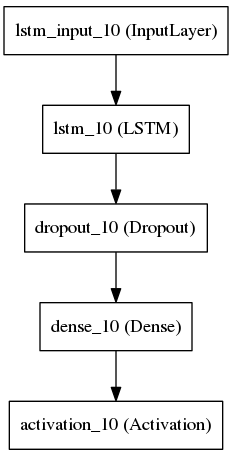
\includegraphics[width=0.7\linewidth]{model}
                \caption{LSTM RNN model implemented}
                \label{fig_model}
            \end{figure}
        \end{columns}
    \end{alertblock}
\end{frame}

%-------------------------------------------------
%   WHY
%-------------------------------------------------
\begin{frame}{Experiment}
    \begin{alertblock}{Training}
    \begin{itemize}
        \item The network is trained one store at a time, each for 5 epochs and 20\% of the data left out for validation
        \item Used mean square error as loss function
    \end{itemize}
    \end{alertblock}

    \begin{table}
        \begin{tabular}{lc}
            \toprule
            Store  & Validation accuracy (\%)\\
            \toprule
            854    & 88.36 \\
            1022   & 71.02 \\
            463    & 82.54 \\
            905    & 93.65 \\
            494    & 99.47 \\
            320    & 86.24 \\
            45     & 99.20\\
            307    & 72.09\\
            \bottomrule
        \end{tabular}
        \caption{Validation accuracy on normalized number of sales}
    \end{table}
\end{frame}

%-------------------------------------------------
%   WHY
%-------------------------------------------------
\begin{frame}{Experiment}
    \begin{figure}[t!]
        \centering
        \begin{subfigure}[t]{0.5\textwidth}
            \centering
            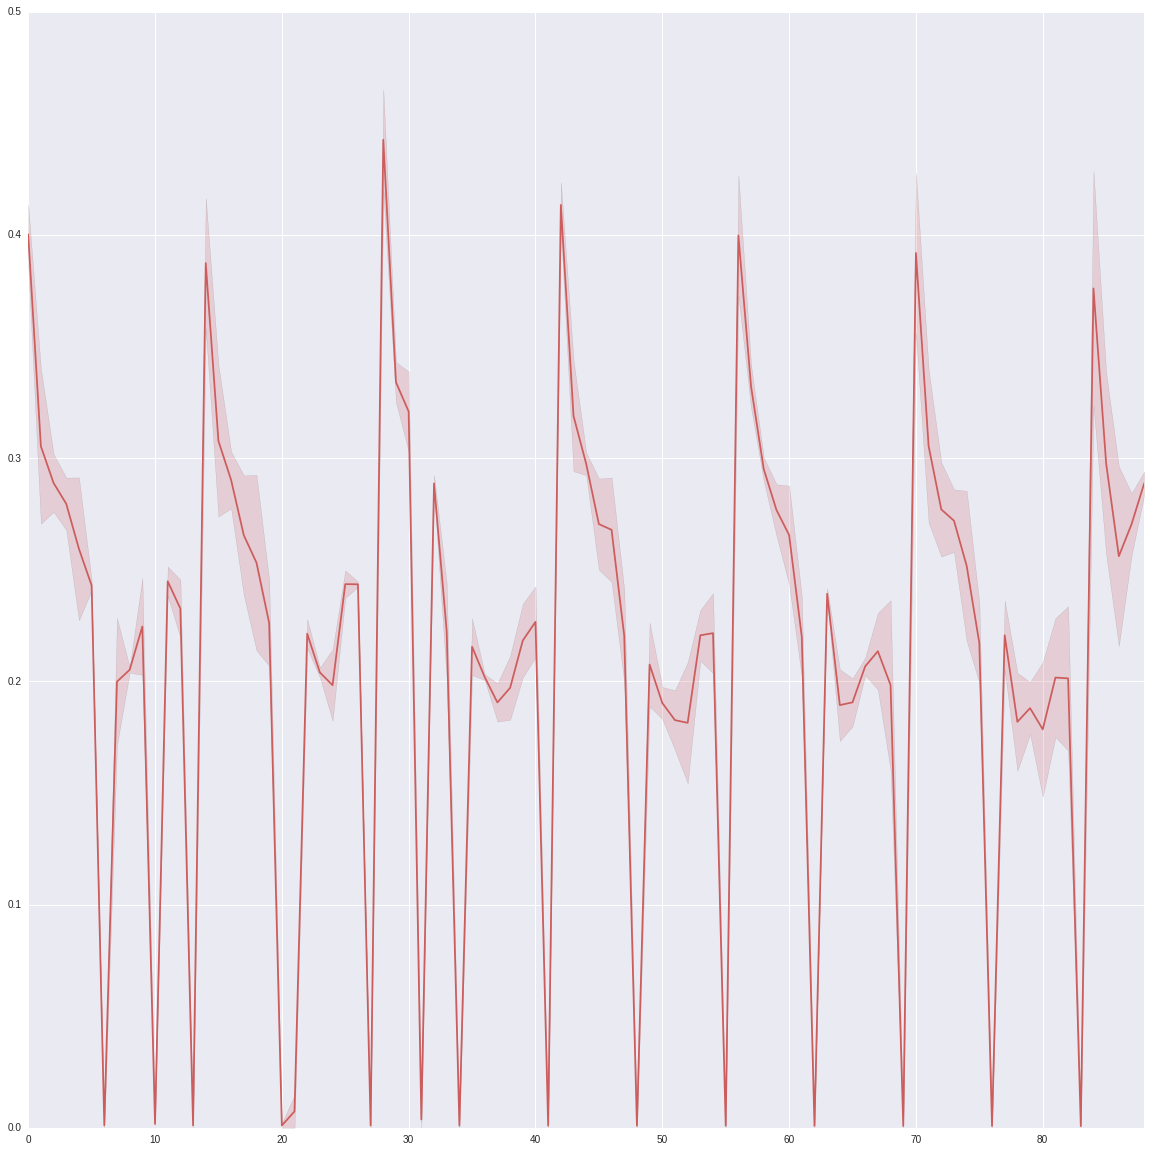
\includegraphics[height=1.5in]{rossmann_prediction_errors_store1022}
            \caption{Store 1022 (71.02\% val acc)}
        \end{subfigure}%
        \begin{subfigure}[t]{0.5\textwidth}
            \centering
            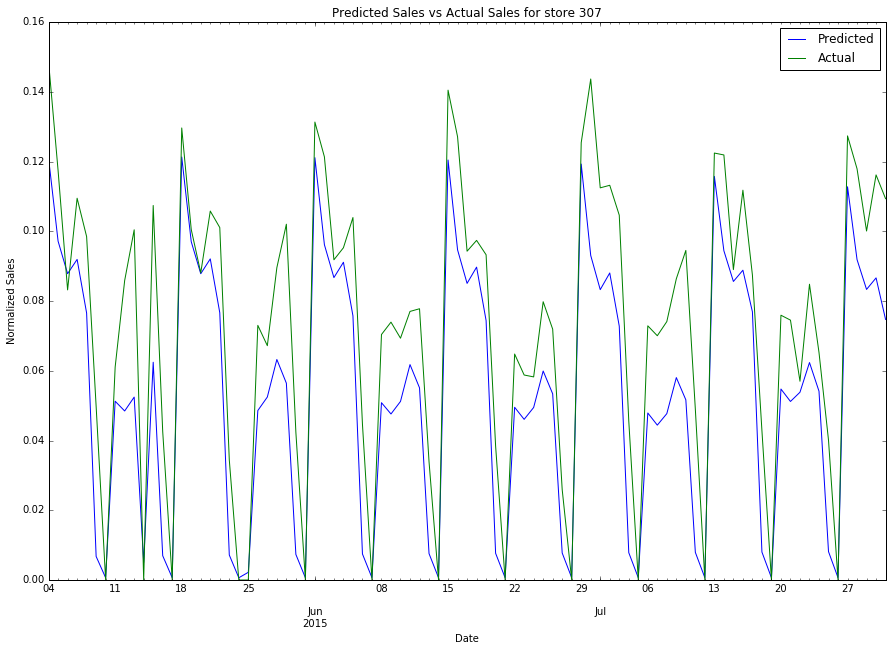
\includegraphics[height=1.5in]{rossmann_prediction_errors_store307}
            \caption{Store 307 (72.09\% val acc)}
        \end{subfigure}
        \label{fig:sub1}
        \caption{Normalized actual and predicted number of sales}
    \end{figure}
\end{frame}

%-------------------------------------------------
%   WHY
%-------------------------------------------------
\begin{frame}{Experiment}
    \begin{figure}[t!]
        \centering
        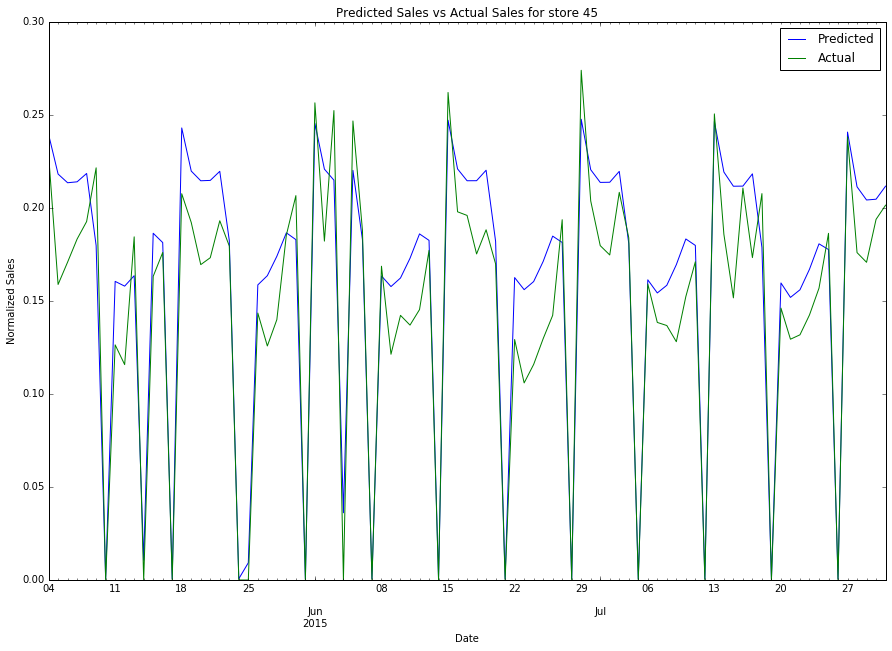
\includegraphics[height=2.6in]{rossmann_prediction_errors_store45}
        \caption{Normalized actual and predicted number of sales for store 45 (99.20\% val acc)}
    \end{figure}
\end{frame}

%-------------------------------------------------
%   WHY
%-------------------------------------------------
\begin{frame}{What's next}
    \begin{itemize}
        \item Use machine learning to fill missing values
        \item Confirm whether using the same model for all the stores is better than training each store separately.
        \item Experiments with more models: more layers and hidden units
        \item Experiment with GRU
        \item Gradually decreasing learning rates
    \end{itemize}
\end{frame}

%-------------------------------------------------
%   END
%-------------------------------------------------
\end{document}
